\documentclass{ctexart}

\title{\Large 移位寄存器及应用\\{\large 实验报告}}
\author{\large  信息科学技术学院 \quad 吴海\MyFont{垚} PB22051035 \\\large  信息科学技术学院 \quad 李\quad 毅 PB22051031 \\{教室:电四楼112室\quad 座位号:12}}
\date{2023年4月1日}
\usepackage{ctex}
\setCJKfamilyfont{myfont}{SimSun.ttf}
\newcommand{\MyFont}{\CJKfamily{myfont}}
\usepackage{amsmath}
\usepackage{amsfonts}
\usepackage{amssymb}
\usepackage{bm}
\usepackage{enumerate}
\usepackage{geometry}
\geometry{left=2.5cm,right=2.5cm,top=2cm,bottom=2cm}
\usepackage{fancyhdr}
\usepackage{lastpage}
\usepackage{booktabs}
\pagestyle{fancy}
\fancyhead[l]{ }
\fancyhead[r]{ }
\fancyhead[C]{
	\begin{tabular}{cclclc}
         & \multicolumn{4}{c}{\textbf{移位寄存器及应用 \quad 实验报告}}                                    &            \\
信息科学技术学院 & \multicolumn{2}{c}{PB22051035 吴海\MyFont{垚}} & \multicolumn{2}{c}{PB22051031 李毅} & 2024年4月1日
\end{tabular}
}
\fancyfoot[C]{ 第 {\thepage} 页,共 \pageref{LastPage} 页}
\renewcommand{\headrulewidth}{2pt}
\usepackage{graphicx}
\usepackage{geometry}
\usepackage[hidelinks]{hyperref}
\usepackage{multicol}
\usepackage{multirow}
\usepackage{ragged2e}
\usepackage[square,comma,numbers,super]{natbib}
\bibliographystyle{unsrt}
\usepackage{siunitx}
\usepackage{subfigure}
\usepackage{wrapfig}
\usepackage{xcolor}
\usepackage{cite}
\begin{document}
    \maketitle
    \thispagestyle{empty}
    
    \newpage 
    \setcounter{page}{1}

    \section*{第一部分 \quad 实验目的}

\begin{enumerate}
    \item 进一步掌握时序逻辑电路的设计步骤和方法
    \item 熟悉和了解移位寄存器的工作原理功能及应用方法
    \item 熟悉中规模4位双向移位寄存器的逻辑功能
\end{enumerate}

    \section*{第二部分 \quad 实验原理}
   \subsection*{1.D触发器}
   本实验使用D触发器搭建寄存器,D触发器特性方程为$Q^*=D$。其结构如图2.1所示

    \begin{minipage}[c]{0.9\textwidth}
        \centering
        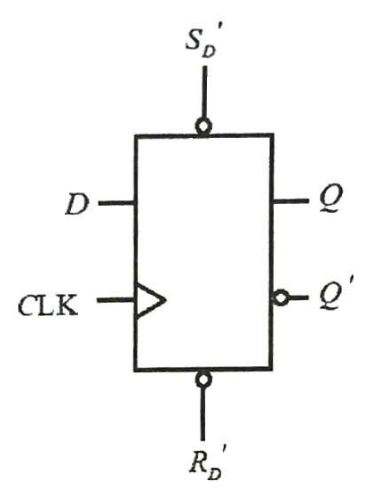
\includegraphics[width=0.4\linewidth]{2.1.png} 

        图2.1 D触发器
    \end{minipage}

    \subsection*{2.移位寄存器}
    移位寄存器是指寄存器中所存的代码能够在移位脉冲的作用下依次左移或右移。既能左移又能右移的移位寄存器称为双向移位寄存器。

    根据存取信息的不同,移位寄存器可以分为:串入串出,串入并出,并入串出,并入并出四种形式。

    图2.2为移位寄存器逻辑电路示例:

    \begin{minipage}[c]{0.9\textwidth}
        \centering
        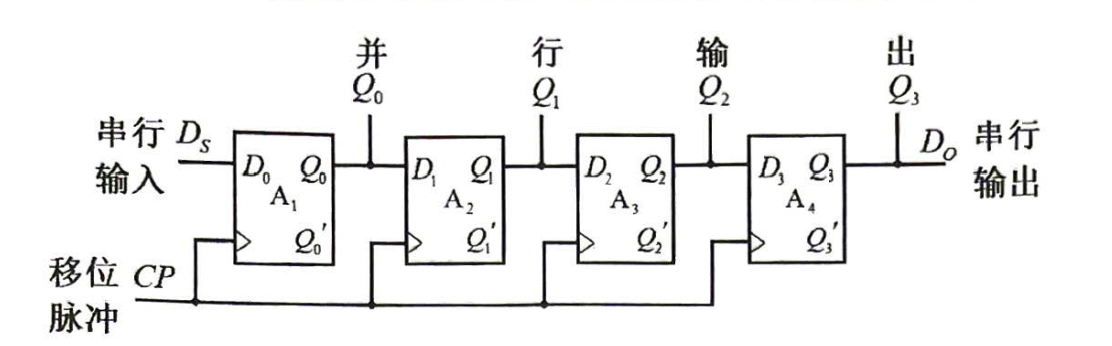
\includegraphics[width=\linewidth]{2.3.png} 

        图2.2 移位寄存器逻辑电路示例
    \end{minipage}

    \subsection*{3.中规模双向移位寄存器}
    中规模双向移位寄存器74LS194如图2.3所示:

    \begin{minipage}[c]{0.9\textwidth}
        \centering
        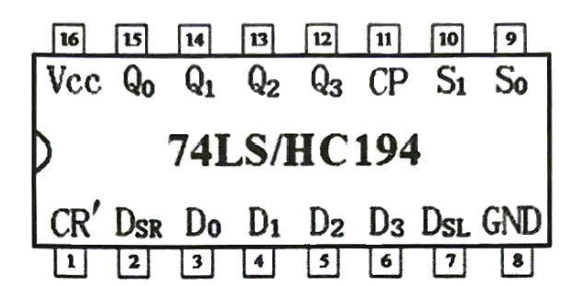
\includegraphics[width=0.7\linewidth]{2.4.png} 

        图2.3 中规模双向移位寄存器74LS194
    \end{minipage}

~\\
    其中$D_0$、$D_1$、$D_2$、$D_3$为并行输入端,$Q_0$、$Q_1$、$Q_2$、$Q_3$为并行输出端。$D_{SR}$为右移串行输入端,$D_{SL}$为左移串行输入端,$S_1$、$S_0$为操作模式控制端,$CR'$为异步清零端,$CP$为移位脉冲输入端。

    其功能表如表1所示:

    \begin{table}[!ht]
    \centering
    表1:74LS194逻辑功能表
    
    \resizebox{0.6\textwidth}{!}{
    \begin{tabular}{|c|c|c|c|c|}
    \hline
    $CP$       & $CR'$ & $S_1$ & $S_0$ & 功能               \\ \hline
    x          & 0     & x     & x     & 清零               \\ \hline
    $\uparrow$   & 1     & 1     & 1     & 并行送数寄存           \\ \hline
    $\uparrow$   & 1     & 0     & 1     & 右移(从$Q_0$到$Q_3$) \\ \hline
    $\uparrow$    & 1     & 1     & 0     & 左移(从$Q_3$到$Q_0$) \\ \hline
    $\uparrow$   & 1     & 0     & 0     & 保持               \\ \hline
    $\downarrow$  & 1     & x     & x     & 保持               \\ \hline
    \end{tabular}
    }
    \end{table}

    \newpage
    \section*{第三部分 \quad 实验内容}
    \subsection*{1.用四块D型触发器接成4位输出的移动寄存器(逻辑电路图如下图所示)}
    \begin{figure}[htbp]
        \centering
        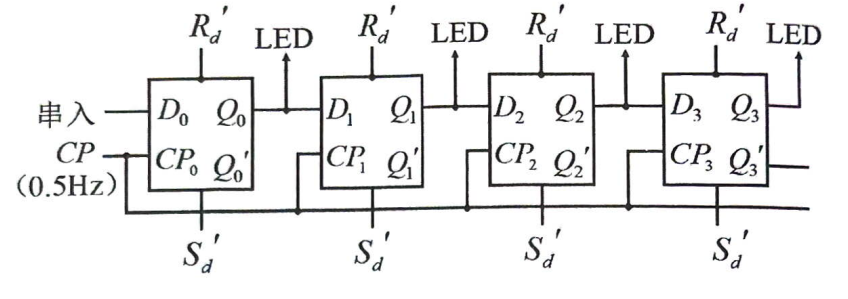
\includegraphics[width=14cm]{3.1.png}
    \end{figure}
    \begin{enumerate}[(1)]
        \item 从$D_0$端串行输入,将寄存器的初态分别置为$Q_3—Q_0$: 0001 , 0110 , 0101 , 0111 在每种初态下,把$D_0$接$Q_3$,记录在CP作用下LED的工作状态。
        \item 从$D_0$端串行输入,将寄存器的初态分别置成$Q_3—Q_0$: 0000 和 0101 ,把$D_0$接$Q_3'$记录在CP作用下LED的工作状态。
        \item 设置自启动函数为:$D_0=((Q_1Q_2')'Q_3)'$记录在CP作用下LED的所用工作状态。
    \end{enumerate}
实验状态转换图记录如下:
    
\noindent (1)\qquad \qquad \qquad \quad 当$Q_3Q_2Q_1Q_0$=0001时     \qquad \qquad \qquad \qquad\qquad 当$Q_3Q_2Q_1Q_0$=0110时
    
    \begin{minipage}[c]{0.5\textwidth}
        \centering
        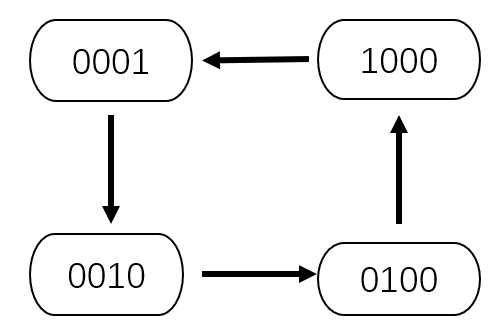
\includegraphics[width=0.75\linewidth]{3.1.1.png} 
    \end{minipage}
    \begin{minipage}[c]{0.45\textwidth}
        \centering
        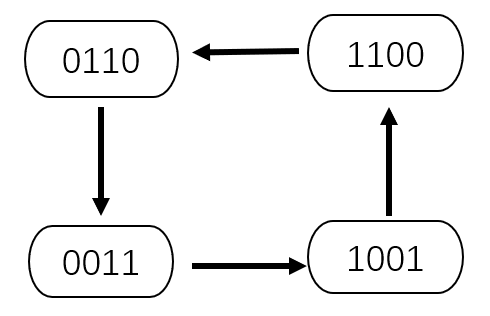
\includegraphics[width=0.8\linewidth]{3.1.2.png} 
    \end{minipage}

   \qquad \qquad \qquad  当$Q_3Q_2Q_1Q_0$=0101时     \qquad \qquad \qquad \qquad\qquad 当$Q_3Q_2Q_1Q_0$=0111 时

    
    \begin{minipage}[c]{0.5\textwidth}
        \centering
        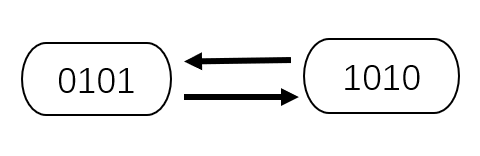
\includegraphics[width=0.8\linewidth]{3.1.3.png} 
    \end{minipage}
    \begin{minipage}[c]{0.45\textwidth}
        \centering
        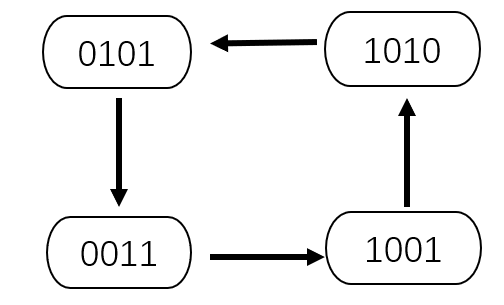
\includegraphics[width=0.8\linewidth]{3.1.4.png} 
    \end{minipage}
    \newpage
    (2)\qquad \quad \qquad  当$Q_3Q_2Q_1Q_0$=0000时     \qquad \qquad \qquad \qquad\qquad 当$Q_3Q_2Q_1Q_0$=0101 时
    
    \begin{minipage}[c]{0.5\textwidth}
        \centering
        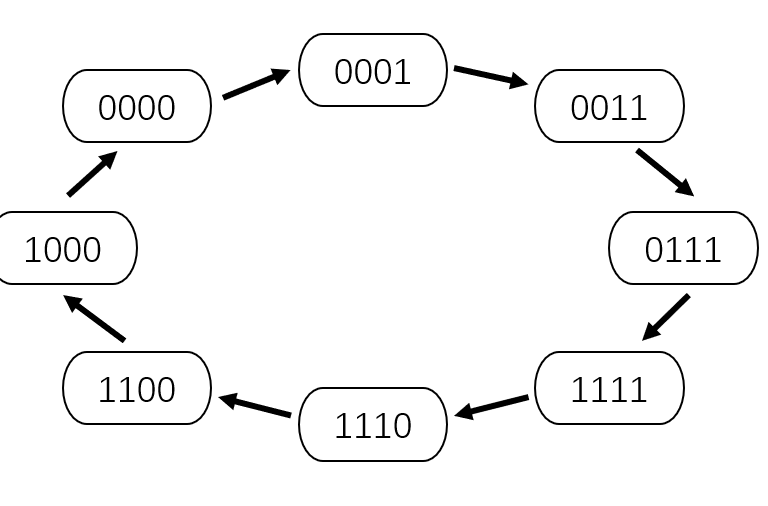
\includegraphics[width=0.78\linewidth]{3.1.5.png} 
    \end{minipage}
    \begin{minipage}[c]{0.45\textwidth}
        \centering
        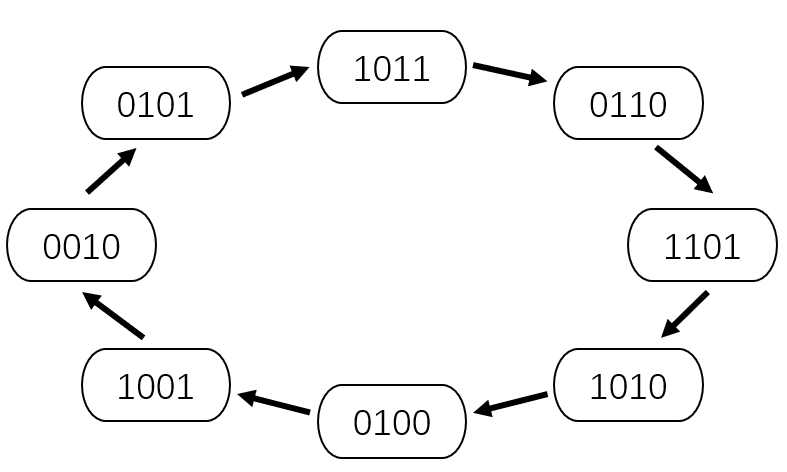
\includegraphics[width=0.8\linewidth]{3.1.6.png} 
    \end{minipage}

    (3)$Q_3Q_2Q_1Q_0$的全状态转化图:
    \begin{figure}[htbp]
        \centering
        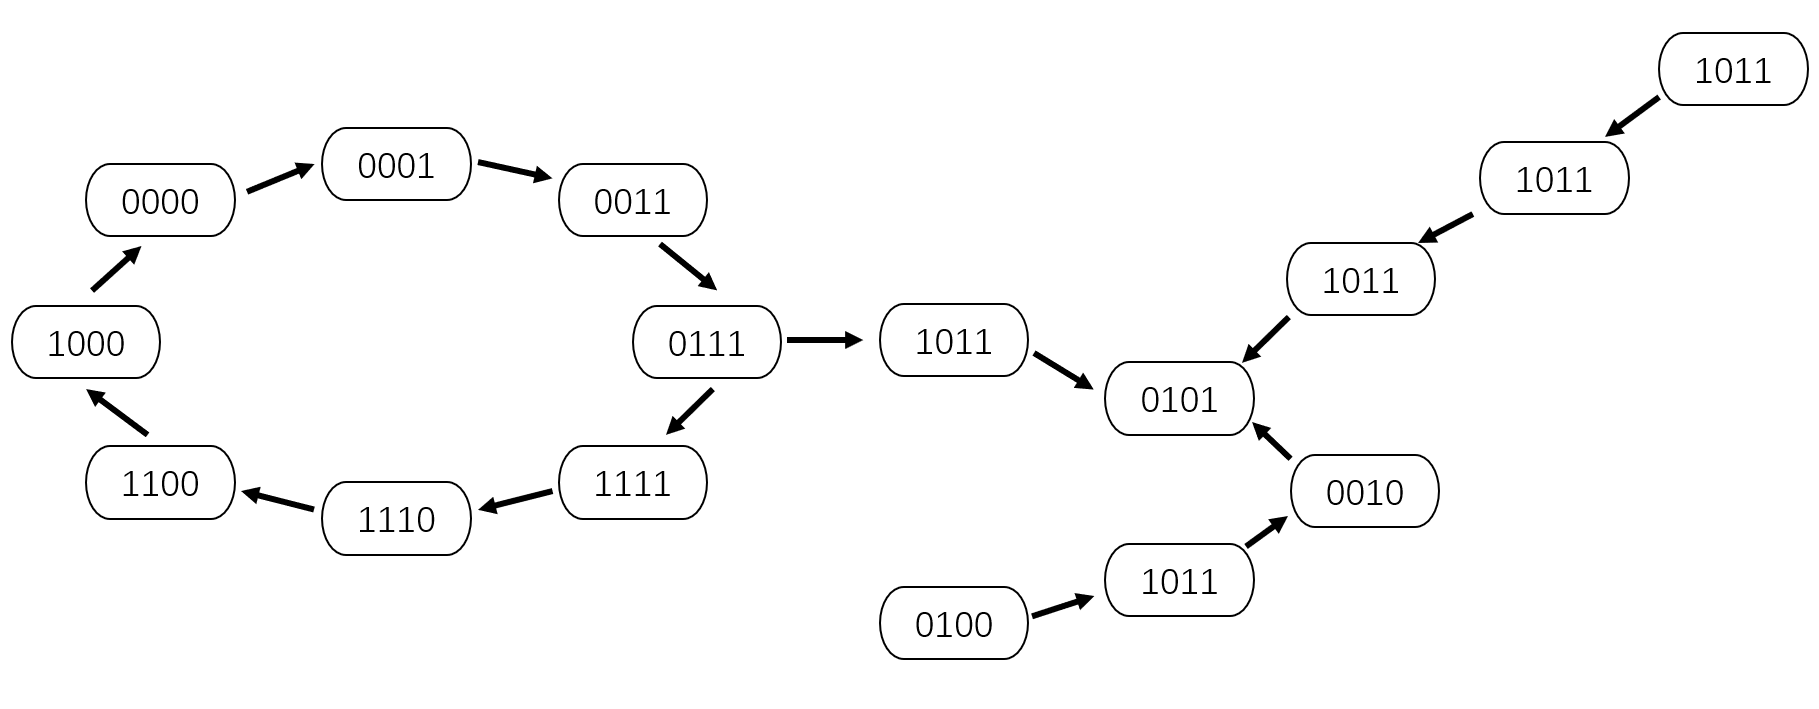
\includegraphics[width=15cm]{3.1.7.png}
    \end{figure}

    \subsection*{2.测试双向移位寄存器的逻辑功能}
    将74LS194清零端CR’接1,$D_0,D_1,D_2,D_3,S_1,S_2$分别接6个逻辑开关,CP接1Hz脉冲信号,$Q_3Q_2Q_1Q_0$分别接4个LED,将$S_0,S_1$分别接四个状态,记录$Q_3Q_2Q_1Q_0$的工作状态


    (1)当$D_0D_1D_2D_3$=0110 时,$Q_3Q_2Q_1Q_0$=0110

       当$D_0D_1D_2D_3$=1001 时,$Q_3Q_2Q_1Q_0$=1001

       因此其置位功能有效。

    (2)测试前后发现,$D_0D_1D_2D_3$与$Q_3Q_2Q_1Q_0$状态一样,芯片保持功能有效

    (3)其状态转化图如下图所示:
    
    \begin{figure}[htbp]
        \centering
        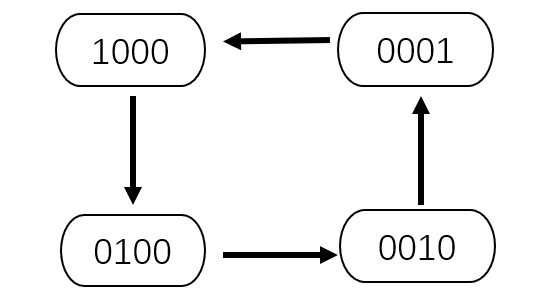
\includegraphics[width=8cm]{3.2.1.png}
    \end{figure}

    (4)其状态转化图如下图所示:
    
    \begin{figure}[htbp]
        \centering
        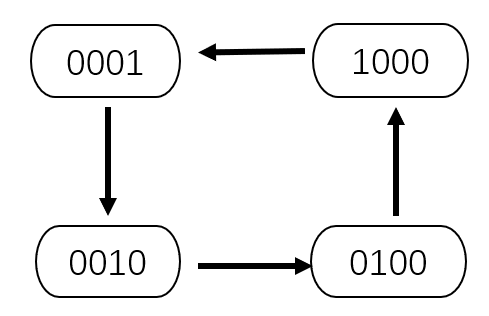
\includegraphics[width=8cm]{3.2.2.png}
    \end{figure}

    \newpage
    \subsection*{3.用74LS194组成包含启动开关的3位串并转换电路}
    使用74LS194设计电路,使得开关置1时进入右移状态,并能循环输出数据$N_3N_2N_10N_3N_2N_10...$
    
    设计电路图如下图所示:
    
    \begin{figure}[htbp]
        \centering
        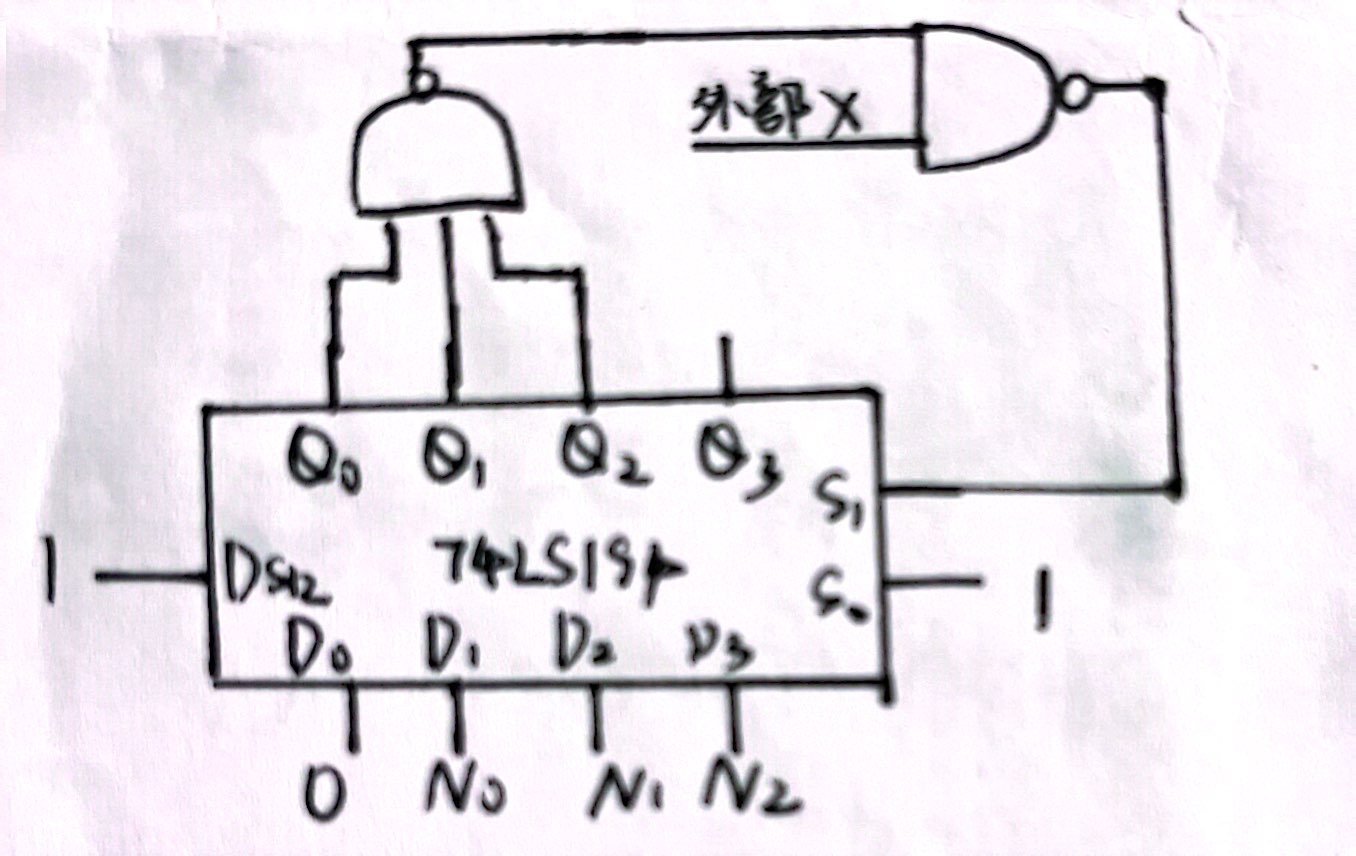
\includegraphics[width=10cm]{3.3.1.jpg}
    \end{figure}

    全状态转化图如下图所示:
     \begin{figure}[htbp]
        \centering
        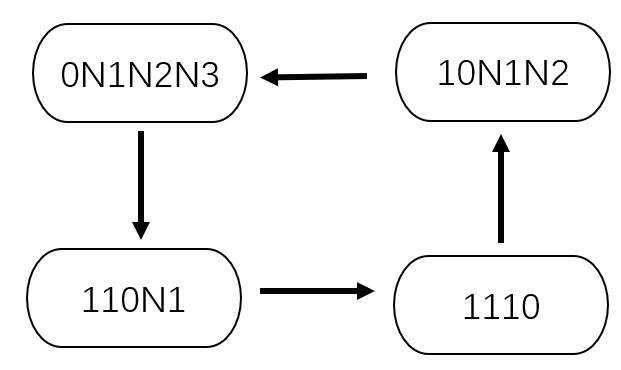
\includegraphics[width=8cm]{3.3.2.png}
    \end{figure}

    输出端循环输出:$N_3N_2N_10N_3N_2N_10...$

    \subsection*{4.用74LS194和74LS151实现能自启动的左移环形计数器。}
    \newpage
    设计电路图如下所示;
    
    \begin{figure}[htbp]
        \centering
        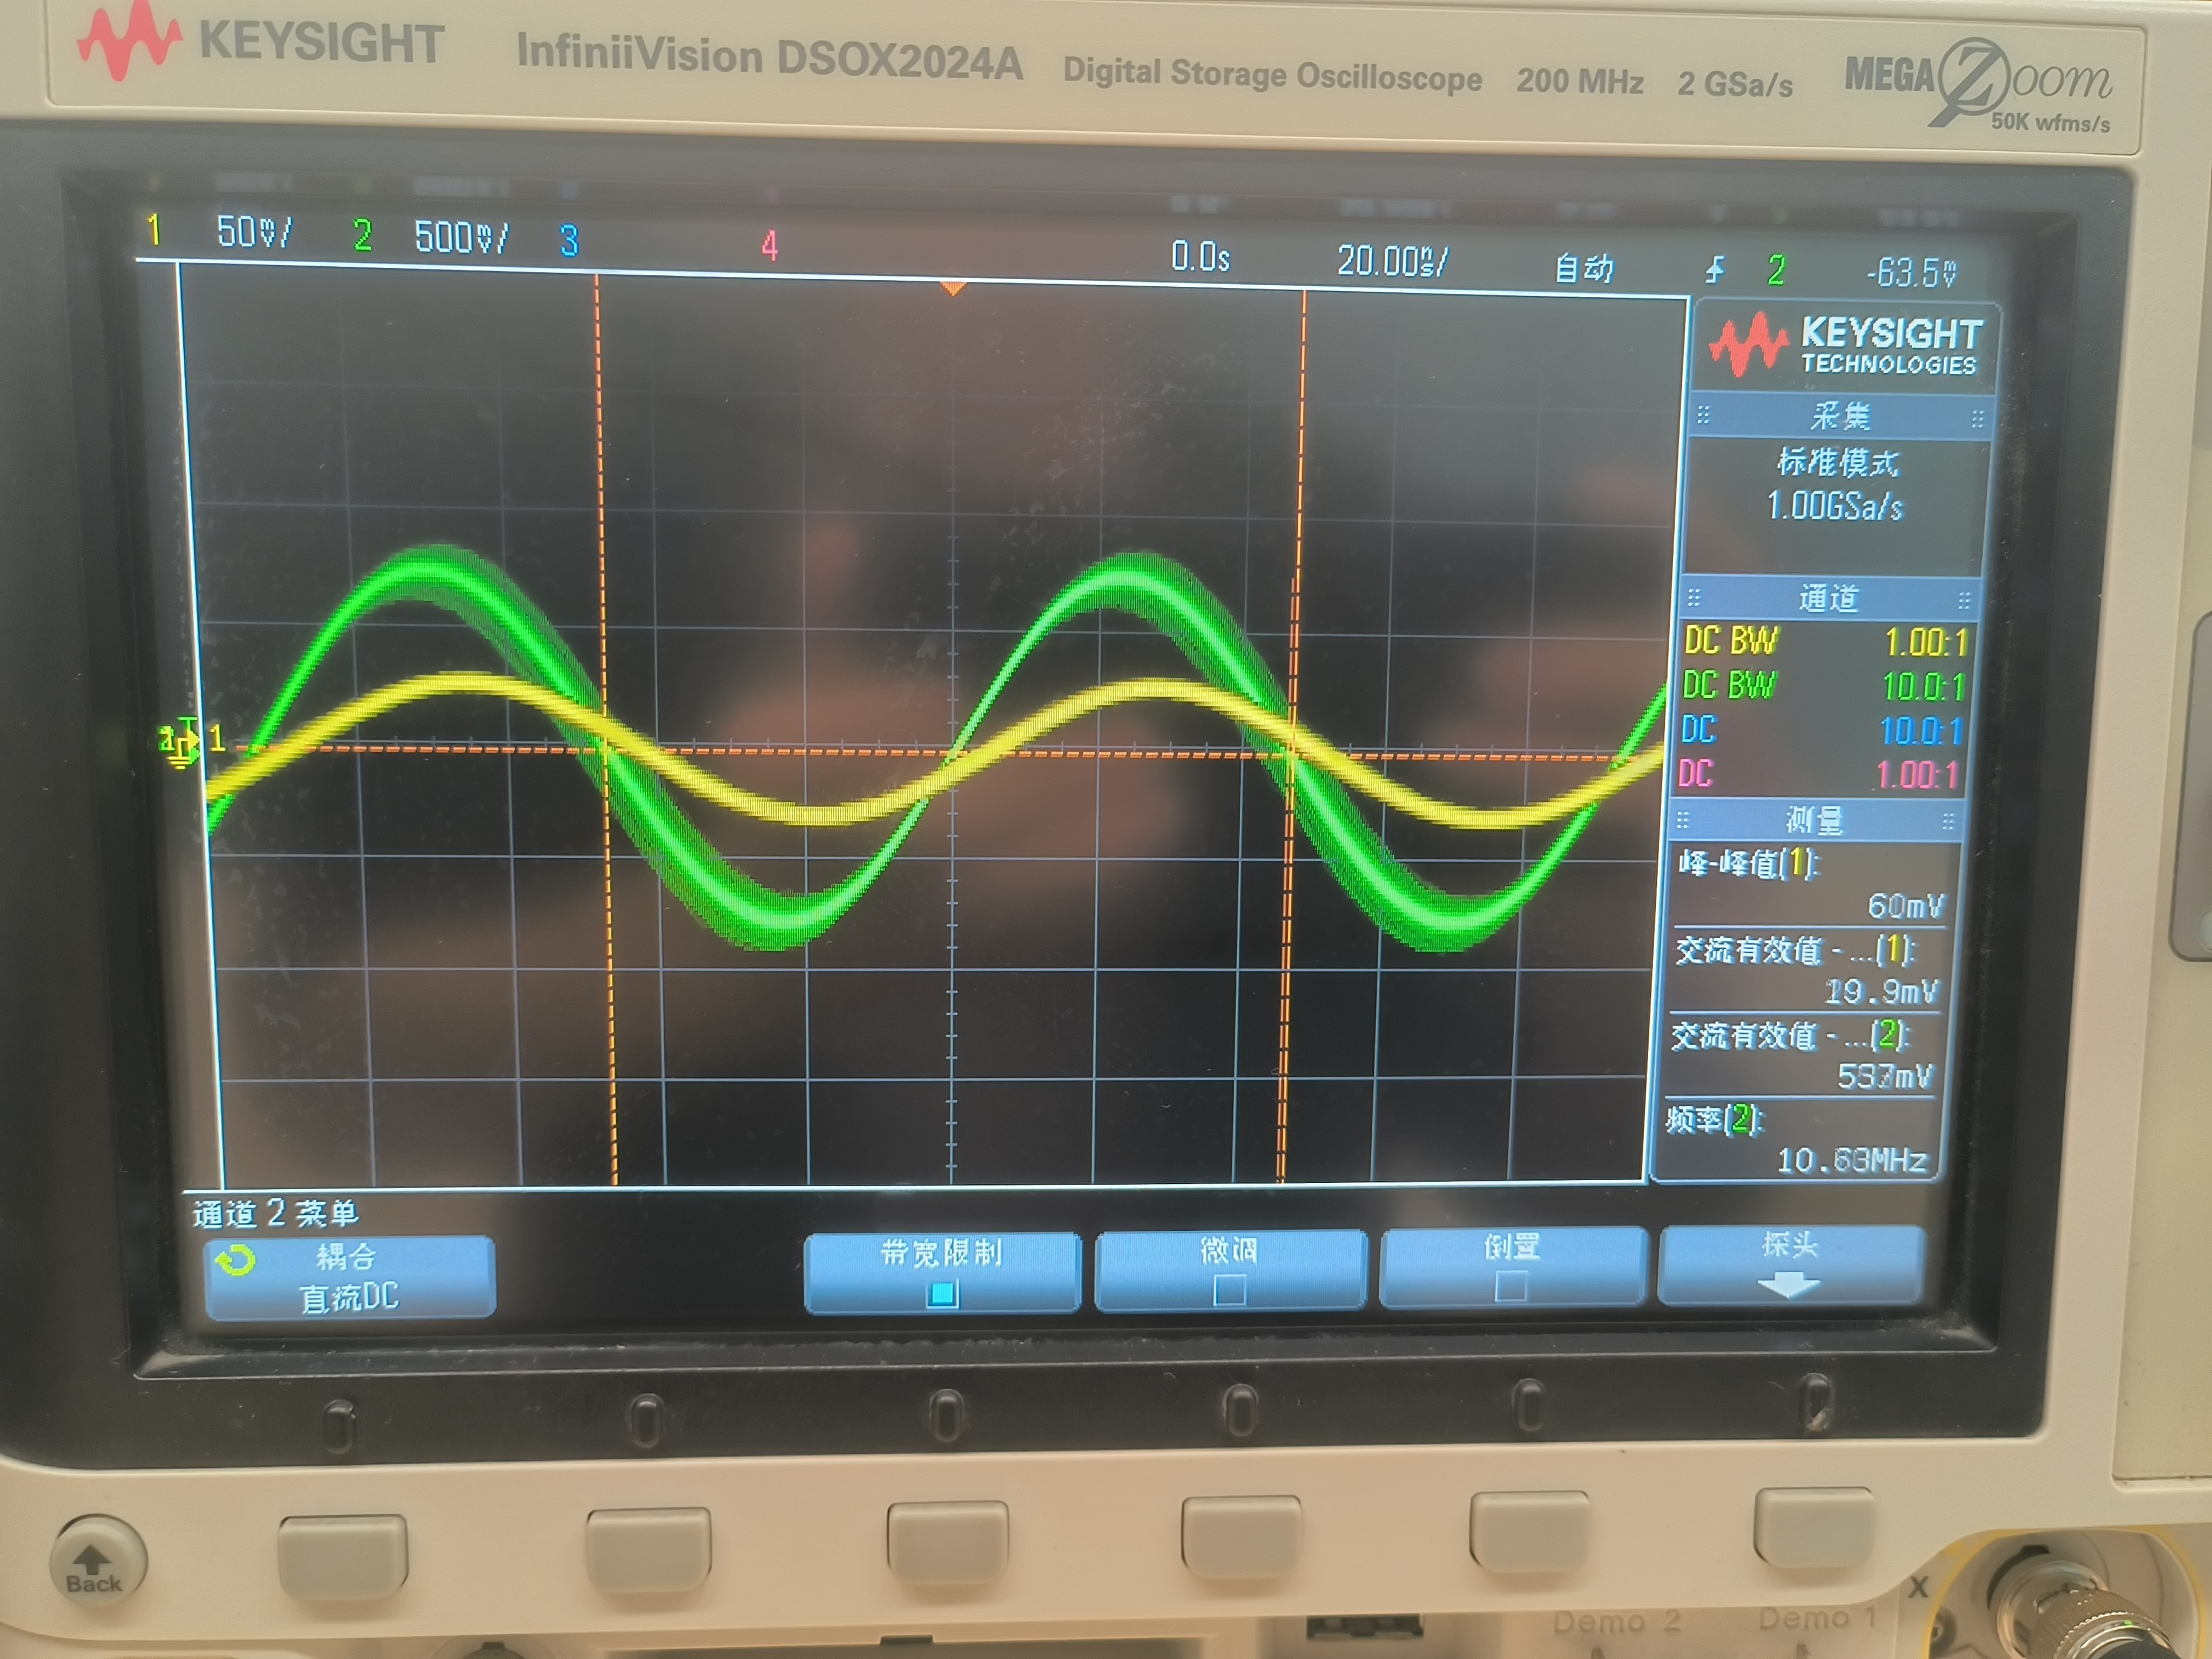
\includegraphics[width=10cm]{3.4.1.jpg}
    \end{figure}

    全状态转化图如图所示:
    
    \begin{figure}[htbp]
        \centering
        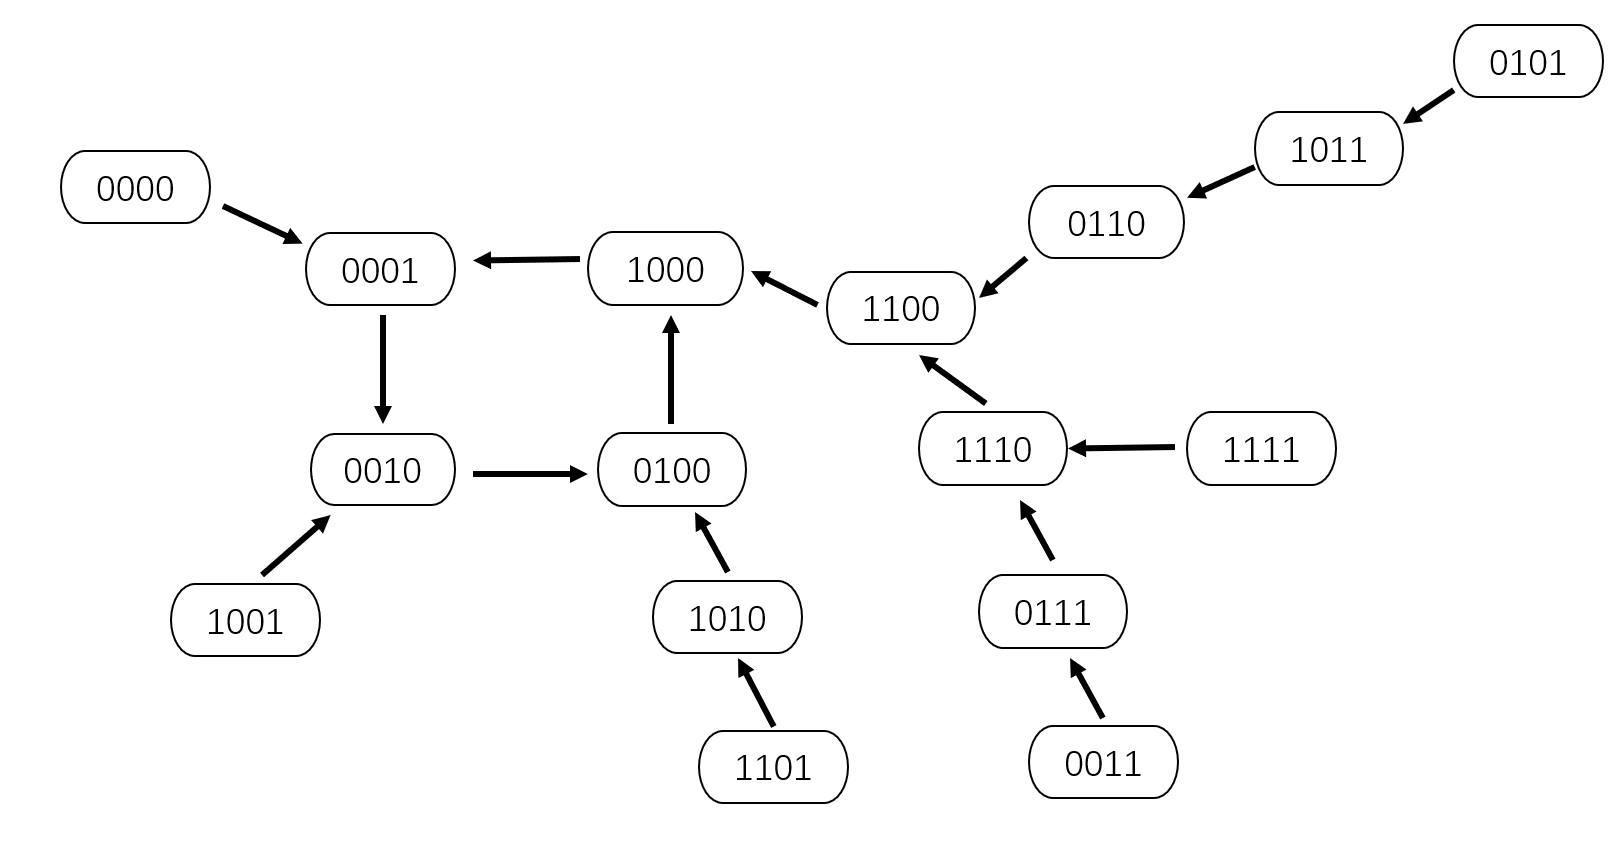
\includegraphics[width=15cm]{3.4.2.png}
    \end{figure}
  

   
    \section*{第四部分 \quad 思考题}
    \subsection*{1.在N位移位寄存器中,串行输入N位二进制数需要多少个CP?送数的次序应从高位至低位,还是低位至高位?}
    
    每一个CP进行一次右移并送数。故串行输入N位二进制数需要N个CP。送数的次序应为从高位至低位。

    \subsection*{2.用74LS194及逻辑门实现一个按7->14->13->11循环计数的自启动四位环形计数器。写出设计过程,画出逻辑图}
    设计状态转换卡诺图(对应$Q^*_3$,$Q^*_2$,$Q^*_1$,$Q^*_0$)如下:
    \begin{table}[!ht]
    \centering
    \begin{tabular}{|c|c|c|c|c|}
    \hline
    $Q_3Q_2/Q_1Q_0$ & 00   & 01   & 11   & 10   \\ \hline
    00              & xxxx & xxxx & xxxx & xxxx \\ \hline
    01              & xxxx & xxxx & 1110 & xxxx \\ \hline
    11              & xxxx & 1011 & xxxx & 1101 \\ \hline
    10              & xxxx & xxxx & 0111 & xxxx \\ \hline
    \end{tabular}
    \end{table}

    x表示无关项。为保证能自启动,设定无关项$Q^*_3$,$Q^*_2$,$Q^*_1$,$Q^*_0$的值,如下表:
    
    \begin{table}[!ht]
    \centering
    \begin{tabular}{|c|c|c|c|c|}
    \hline
    $Q_3Q_2/Q_1Q_0$ & 00   & 01   & 11   & 10   \\ \hline
    00              & 0001 & 0011 & 0111 & 0101 \\ \hline
    01              & 1001 & 1011 & 1110 & 1101 \\ \hline
    11              & 1001 & 1011 & 1110 & 1101 \\ \hline
    10              & 0001 & 0011 & 0111 & 0101 \\ \hline
    \end{tabular}
    \end{table}

    由此画出状态转换图(对应$Q_3$$Q_2$$Q_1$$Q_0$)如下:
    
    \begin{minipage}[c]{0.9\textwidth}
        \centering
        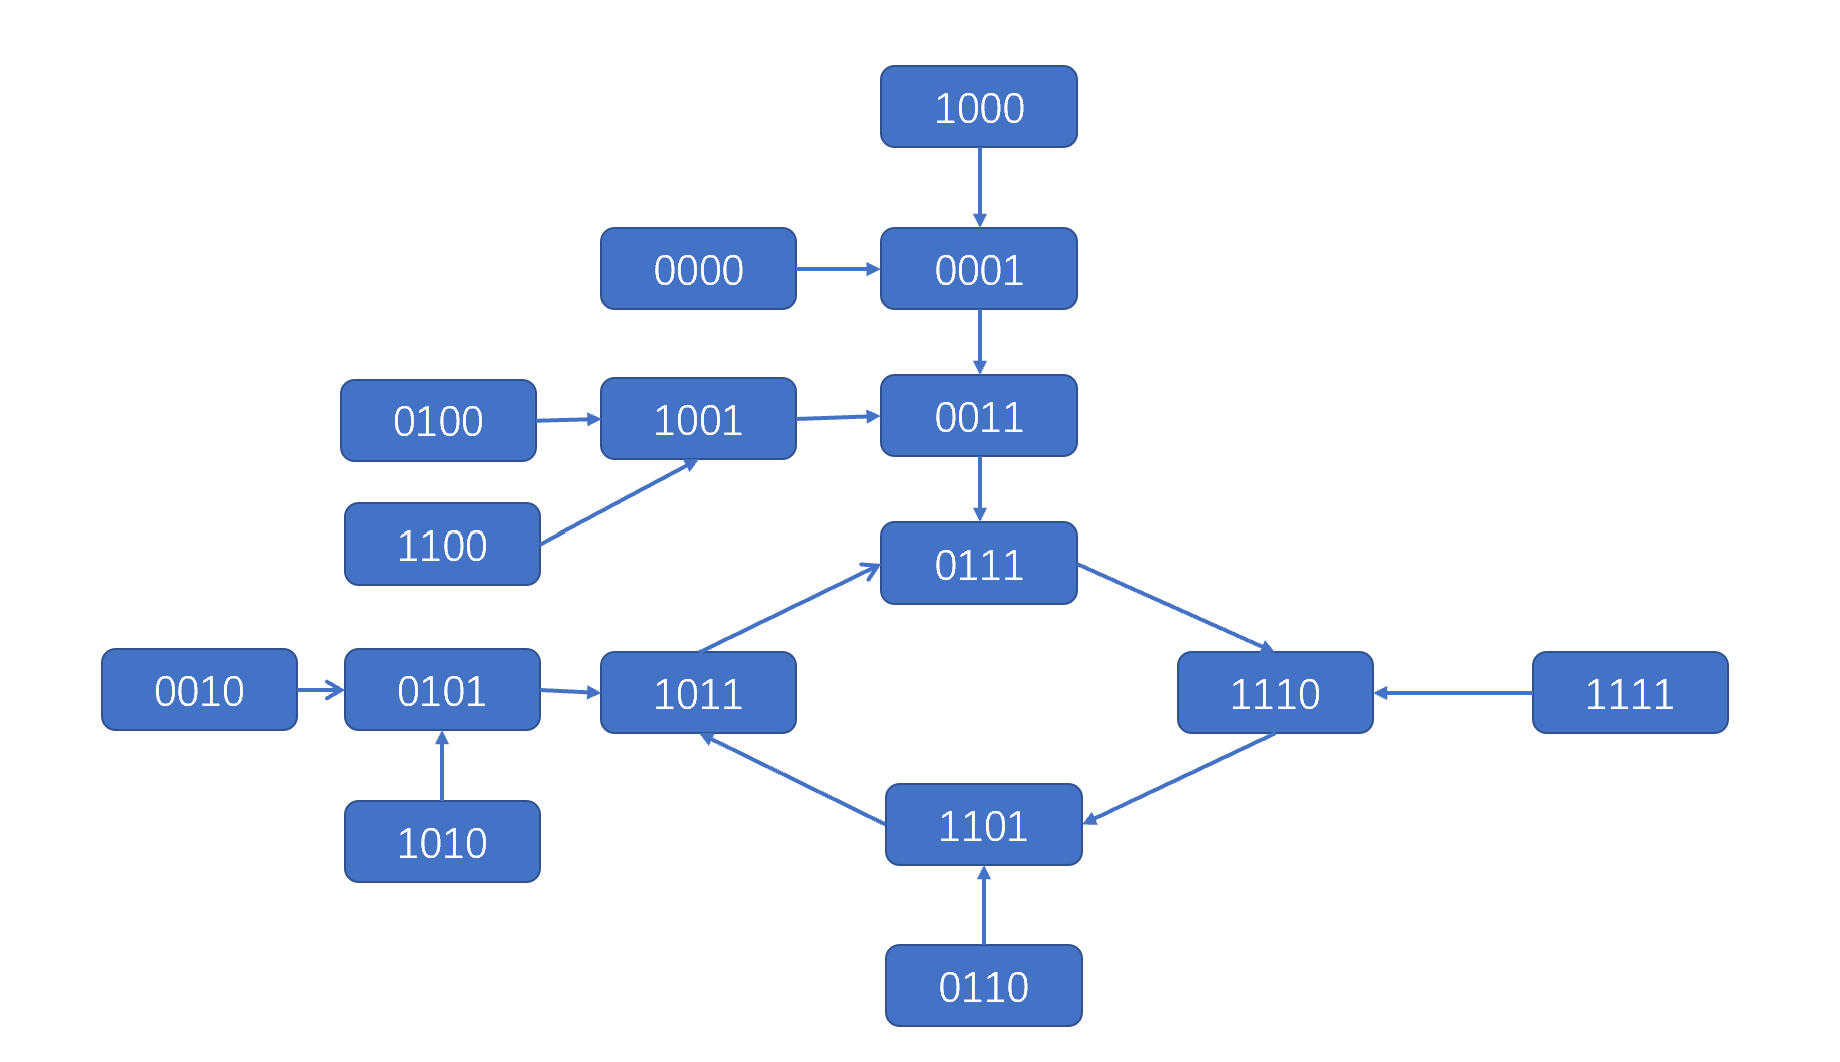
\includegraphics[width=\linewidth]{思考题.png} 
    \end{minipage}

    写出状态方程:
    $$Q^*_3=Q_2$$
    $$Q^*_2=Q_1$$
    $$Q^*_1=Q_0$$
    $$Q^*_0=Q'_2+Q'_1+Q'_0$$

    74LS194设定右移模式(方向从$Q_0$到$Q_3$)时,$Q^*_0Q^*_1Q^*_2Q^*_3=D_{SR}Q_0Q_1Q_2$,故$D_{SR}=Q^*_0=Q'_2+Q'_1+Q'_0=(Q_2Q_1Q_0)'$,为驱动方程。

    画出电路图如下:

    \begin{minipage}[c]{0.9\textwidth}
        \centering
        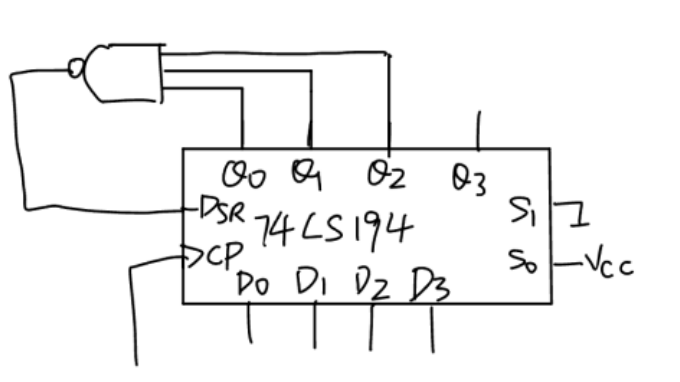
\includegraphics[width=\linewidth]{思考题2.png} 
    \end{minipage}

    
    
\end{document}
